\textsl{
Bien avant qu'elle ne soit conceptualisée, on a utilisé des itérations où est sous-jacente la notion de suite. Par exemple, \textsc{Archimède} quand il cherche une valeur approchée de $\pi$ considère les suites $(p_n)$ et $(P_n)$ des périmètres des polygones inscrits et circonscrits à un cercle de rayon $1$ et aboutit à des formules qui équivalent à $p_{2n} = \sqrt{p_n P_n}$ et $P_{2n} = \frac{2 P_n p_{2n}}{p_{2n} + P_n}$. \\
La théorie des suites au sens moderne est établie au début au début du \textsc{xix}$^\me$ siècle quand s'affirme la volonté de donner à l'analyse des bases rigoureuses qui la débarrassent des notions métaphysiques d'infiniment petits ou de quantités évanouissantes. Dans ses \emph{Notions fondamentales de la théorie des suites}, rédigée vers 1800 et restées inédites, \textsc{Gauss} donne la définition moderne d'une suite (application de $\N$ dans $\R$). Il définit les notions de majorant et de borne supérieure d'une suite. Plus intéressant encore, il donne les définitions de la limite supérieure et de la limite inférieure d'une suite ($\lim \sup a_n = \lim\limits_{n \to + \infty} \sup\limits_{p \geqslant n} a_p$ et $\lim \inf a_n = \lim\limits_{n \to + \infty} \inf\limits_{p \geqslant n} a_p$, dans le langage d'aujourd'hui) et, quand ces deux quantités sont égales, appelle leur valeur commune la limite de la suite. \\
C'est le \emph{Cours d'analyse} de \textsc{Cauchy} (1821) qui ouvre la voie à l'analyse moderne. Dans le chapitre des \emph{Préliminaires}, il donne les définitions d'une suite et de la limite d'une suite, les premières définitions précises de $+\infty$ et $-\infty$, introduit la notion de valeur d'adhérence. Le \say{ critère de \textsc{Cauchy} } de convergence, déjà connu de \textsc{Bolzano} est explicité pour les séries. \\
Pendant une grande partie du \textsc{xix}$^\me$ siècle, la convergence d'une suite de \textsc{Cauchy} ou d'une suite croissante majorée sont présentés comme des axiomes qui constituent le fondement de toutes les questions où intervient la notion de limite. Ce point de vue va être remis en cause par \textsc{Méray} (1868) puis par \textsc{Cantor} (1872) qui, voulant en donner des justifications précises, contruisent $\R$ à partir des suites de \textsc{Cauchy} de $\Q$. \\
La théorie des suites réelles dont tous les concepts sont parfaitement définis depuis la fin du \textsc{xix}$^\me$ a connu récemment des développements importants avec l'étude des systèmes dynamiques, qui apportent un regard nouveau sur les suites définies par une relation de récurrence de la forme $u_{n+1} = f(u_n)$. Si la fonction $f$ est continue et si la suite converge, sa limite $\ell$ est nécessairement un point fixe de $f$. Ce fait, démontré par \textsc{Cauchy}, est à la base de toutes les méthodes numériques itératives. L'intérêt pour telles suites est ancien. Dans le traité \emph{De la méthode des fluxions et des suites infinies} (1740), pour obtenir une valeur approchée d'une solution de l'équation $g(x) = 0$. \textsc{Newton} expose ce qu'on appelle depuis \say{ méthode de \textsc{Newton} }: prenant $a_0$ proche de la solution de l'équation, on considère une suite vérifiant 
$$a_{n+1} = a_n - \frac{g(a_n)}{g'(a_n)}.$$
\begin{marginfigure}[-5cm]
    \centering
    % https://tex.stackexchange.com/questions/549225/how-to-make-tangents-on-figure-like-this
\begin{tikzpicture}[scale=0.8, >=stealth,
    declare function={f(\x)=-0.35+5*exp(\x/2)/exp(3);
        fprime(\x)=2.5*exp(\x/2)/exp(3);},
    dot/.style={circle,fill,inner sep=1pt},
    every pin edge/.style={thin}, scale=0.8]
  \path (0,0) coordinate[label=below left:{$O$}] (O)
     (0,5) coordinate (y) (6,0) coordinate (x);
  \draw[-latex,name path=x-axis] (-0.5,0) --  (x) node[below] {$x$};
  \draw[-latex] (0,-0.5) --  (y) node[left] {$g(x)$};
  \draw[semithick,cyan,name path=curve] plot[variable=\x,domain=0.1:6,smooth]
   (\x,{f(\x)}) (5.8,{f(6)});
  \draw[red,dashed] (5.5,0) coordinate(x0) -- (5.5,{f(5.5)}) coordinate(p0)
  ($(p0)+(-1,{-1*fprime(5.5)})$) coordinate(p0');
  \draw[red,dashed] (intersection of p0--p0' and O--x) coordinate (x1)
  let \p1=(x1) in \pgfextra{\pgfmathsetmacro{\myx}{\x1/1cm}}
  (x1) -- (\myx,{f(\myx)}) coordinate(p1)
  ($(p1)+(-1,{-1*fprime(\myx)})$) coordinate(p1');
  \draw[red,dashed] (intersection of p1--p1' and O--x) coordinate (x2)
  let \p1=(x2) in \pgfextra{\pgfmathsetmacro{\myx}{\x1/1cm}}
  (x2) -- (\myx,{f(\myx)}) coordinate(p2)
  ($(p2)+(-1,{-1*fprime(\myx)})$) coordinate(p2');
  \path (intersection of p2--p2' and O--x) coordinate (x3)
    (x3) node[draw,label=below:{$a_{3}$}] {}
  foreach \X [count=\Y] in {0,...,2}
   {(x\X) node[draw,label=below:{$a_{\X}$}] {}
    (x\Y) edge[red,shorten >=-1em,shorten <=-1ex] (p\X)
   \ifnum\X=0   
   (p\X) node[dot,cyan,label={[black]left:{$\big(a_{\X},g(a_{\X}) \big)$}}] {}
   \else
   (p\X) node[dot,cyan,pin={[black]90:{$\big( a_{\X},g(a_{\X}) \big)$}}] {}
   \fi 
   };
  \path[name intersections={of=curve and x-axis,by=i}]
   (i) node[cyan,draw,fill,
   ,pin={[black,align=center]90: point\\ \contour{white}{recherché}}](in){};  
 \end{tikzpicture}

    \caption*{\centering Illustration de la méthode de \textsc{Newton}}
\end{marginfigure}
C'est lors de l'étude de certains systèmes dynamiques discrets \footnote{Qui revient à l'étude du comportement des applications itérées $f^n : X \to X$.} qu'est apparue la notion de chaos, qui a connu ces dernières décennies un grand succès. Pour des fonctions $f$ très simples (par exemple une fonction trinôme), le système dynamique peut avoir un comportement qui semble aléatoire. L'exemple le plus connu est la \emph{suite logistique} vérifiant une relation de la forme
$$u_{n+1} = (1 + \alpha) u_n - \alpha u_n^2.$$
Cette suite a été utilisée par \textsc{Verhulst} en 1845 pour décrire un modèle de croissance de la population. Pour $0 < \alpha \leqslant 2$ et une population $u_0$ pas trop importante, la suite $(u_n)$ converge vers la population stable $1$. Mais comme l'a démontré en 1963 le météorologiste $\textsc{E. N. Lorenz}$, pour des valeurs plus grandes de $\alpha$, cette loi décrit certains aspects des flux turbulents. \\
Dans les années 1980, de grands progrès ont été accomplis dans l'étude de ces systèmes dynamiques grâce à la puissance des ordinateurs. Par exemple, pour la suite logistique, on observe que, pour $2 < \alpha < 2,5$, le comportement de la suite tend vers une oscillation régulière entre deux valeurs (cycle d'ordre $2$); puis pour $2,5 \leqslant \alpha < 2,55$, vers un cycle d'ordre $4$; ensuite quand $\alpha$ augmente, vers des cycles d'ordres $8, 16, \dots$ Au-delà de $2,57$ environ, le système devient chaotique. \textsc{Feigenbaum} a montré en 1981 que, pour une classe assez large d'applications $f$ de $[-1, 1]$ dans $[-1, 1]$ et $f_\lambda = \lambda f, 0 < \lambda < 1$, le système dynamique défini par $u_{n+1} = f_\lambda(u_n)$ a un comportement comparable: il existe une suite croissante de valeurs $\lambda_j$ du paramètre $\lambda$ pour lesquelles la dynamique change (le nombre de points d'un cycle double quand $\lambda$, supposé passage de $\lambda_j$) jusqu'à une valeur critique $\lambda_\infty$, de telle manière que $\frac{\lambda_{j+1} - \lambda_j}{\lambda_{j+2} - \lambda_{j+1}}$ tende vers $\delta = 4,669\dots$, constante universelle indépendante de $f$. Au-delà de $\lambda_\infty$, on retrouve des cycles stables de période $3 \cdot 2^j$ et des points de bifurcation. \\
On s'est aussi intéressé à l'itération de fonction complexes, en particulier les fonction $f : x \mapsto x^2 + c$, où $c \in \C$. On étudie l'ensemble des nombres complexes $z$ pour lesquels la suite de premier terme $z$ est bornée. On note $K_c$ cet ensemble, et on l'appelle \emph{ensemble de \textxsc{Julia}}. Sa frontière présente des formes très belles et très variés selon les valeurs de $c$. Les premiers résultats, établis entre 1905 et 1920, sont dus à \textsc{Fatou} et \textsc{Julia} (évidemment sans aucun moyen informatique). En 1980, \textsc{Mandelbrot} étudia l'ensemble des points $c$ pour lesquels $0$ est dans $K_c$ (le célèbre \emph{ensemble de \textsc{Mandelbrot}}). 
\begin{marginfigure}[-2cm]
    \centering
    \caption*{\centering L'ensemble de \textsc{Mandelbrot}}
    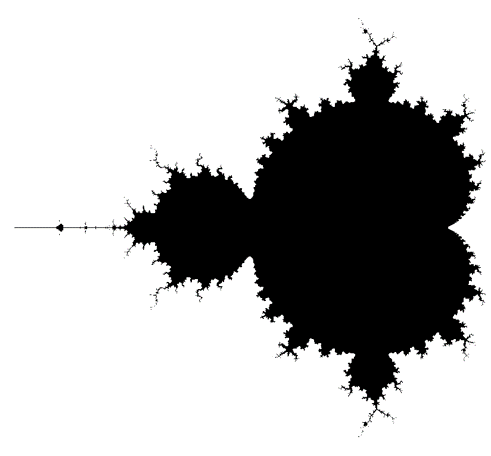
\includegraphics[scale=0.5]{images/ensemble_de_mandelbrot.png}
\end{marginfigure}
Les ensembles de \textsc{Julia} ont les propriétés des fractales, en particulier l'autosimilitude. En revanche, l'ensemble de \textsc{Mandelbrot} est extraordinairement varié: plus l'échelle est grande, plus l'image se complique. On a montré un caractère universel de l'ensemble de \textsc{Mandelbrot}: pour diverses fonctions complexes à un paramètre, on trouve des copies déformées de cet ensemble. 
}

Séries numériques (oraux x-ens)\\
\textsl{
Dans une tentative d'historique des séries numériques, nous pourrions faire remonter leurs origines aux travaux développés dès la fin du \textsc{xvii}$^\me$ siècle autour du comportement asymptotique de sommes du type $\sum\limits_{k=1}^n f(k)$. Quelques années après les travaux de \textsc{Bernoulli} sur ce sujet, \textsc{Euler} et \textxsc{Mac-Laurin} produisent indépendamment une \say{ formule sommatoire } obtenue par inversion d'identités tayloriennes:
$$\sum_{k=1}^n f(k) = \int_0^n f + \frac{f(0) + f(n)}{2!} + \frac{f'(n) - f'(0)}{3!} - \frac{f'''(n) - f'''(0)}{6!}\cdots$$
\marginnote[0cm]{
    \note En notant $\mathrm{b}_k$ les nombres de \textsc{Bernoulli},
    $$\sum_{k=0}^{n-1} k^m = \sum_{k=0}^m \binom{m}{k} \mathrm{b}_k \frac{n^{m+1-k}}{m+1-k}.$$
    Pour $|x| < 2 \pi$,
    $$\frac{x}{\me^x-1} = \sum_{k=0}^{+\infty} \mathrm{b}_k \frac{x^k}{k!}.$$
    \note Soit $s \in \Ne$,
    $$\sum_{n=1}^{+\infty} \frac{1}{n^{2s}} = \frac{|\mathrm{b}_{2s}|(2 \pi)^{2s}}{2 (2s)!}.$$
}
Si l'expression générale donnant les coefficients de cette formule leur échappe dans un premier temps, \textsc{Euler} établit leur lien avec les coefficients du développement en série de $\frac{x}{\me^x-1}$ et les nombres de \textxsc{Bernoulli}, introduits par celui-ci dans le calcul des sommes $\sum\limits_{k=1}^n k^p$ \note. \textxsc{Euler} en déduit, par de jolis calculs, les sommes des séries $\sum\limits_{n=1}^{+\infty} \frac{1}{n^{2s}}$ pour $s$ entier naturel non nul \note.
Cependant, le problème de la convergence des sommes en question n'est jamais au centre de leurs réflexions et l'aspect formel l'emporte, ce qui conduit parfois les plus grands mathématiciens du siècle à commettre de lourdes erreurs. Vers 1768, \textsc{d'Alembert} commence à douter de la validité de l'emploi de séries non convergentes. En 1826, le mot d'\textsc{Abel} illustre parfaitement cette nouvelle préoccupation: \say{ Les séries divergentes sont des inventions du diable, et c'est une honte que l'on ose fonder sur elles la moindre démonstration. On peut en tirer  tout ce qu'on veut quand on les emploie et ce sont elles qui ont produit tant d'échecs et tant de paradoxes } (Œuvres, 1881). \\
Mais ce sont les nécessités du calcul numérique qui imposent vraiment un effort de rigueur dont \textsc{Gauss}, s'étant fait une idée claire de la notion de limite, sera le principal artisan. À partir de là, il paraît naturel d'établir des critères simples de convergence: on en doit plusieurs à \textsc{Cauchy}, et notamment celui qui porte son nom: si la suite de réels positifs $(a_n)_{n \geqslant 0}$ est telle que la limite supérieure de $\sqrt[n]{a_n}$ est strictement inférieure à $1$, alors la série $\sum a_n$ est convergente. \\
(il y a une suite)
}